\documentclass{article}
\input{C:/Users/aryay/OneDrive/Shared Files/Programs/Preamble.tex}


\title{Geodesics using Weight Functions}
\author{Arya Yae}
\date{}

\begin{document}

\maketitle

\section*{The Polar Geodesic Equation}
Let $U\subseteq\C$ be an open region.  In the complex coordinate $z$, a conformal metric has the form $g=u(z)|\de z|^2$ where $u$ is called a \emph{weight function}.  Here $|\de z|^2$ represents the standard complex dot product.  At a point $p\in U$ and a vector $w$ starting at $p$, the norm of $w$ with respect to $g$ is $|w|_g=\sqrt{u(p)}|w|$, where $|w|$ is the standard norm.  Note that we've switched from the earlier convention $g=u^2|\de z|^2$ to match the M.R.S.\ paper.

The connection induced by $g$ is given by $\nabla=\de+\del\log u$.  Evaluating this connection on a function $f$ gives
\begin{equation}
    \nabla f=\de f + (\del_z\log u)f\,\de z
\end{equation}
In the case where $\gamma\from[0,T)\to U$ is a geodesic, we can extend the derivative $\dot\gamma$ to a vector field on a tubular neighborhood of $\im\gamma$.  Since the tangent bundle of $U$ is trivial, a vector field is the same as a complex function.  Thus
\begin{equation}\label{eqn: geodesic equation}
    0=\nabla_{\dot\gamma}\dot\gamma=\ddot\gamma+(\partial_z\log u)\dot\gamma\cdot\langle\de z,\dot\gamma\rangle=\ddot\gamma+(\del_z\log u)\dot\gamma^2,
\end{equation}
where $\langle\de z,\dot\gamma\rangle$ is the duality pairing\footnote{
    In $\C^n$ with coordinates $(z_1,\dots,z_n)$, for a vector $\vec v=(v_1,\dots,v_n)$ the pairing is $\langle\de z_i,\vec v\rangle=v_i$.  In a single dimension where $\vec v$ is just a complex number, it's simply $\langle\de z,v\rangle=v$.
}.  Our weight function will be given in terms of polar coordinates $(r,\theta)$.  Recall
    $$\partial_z=\frac{e^{-i\theta}}{2r}(r\partial_r-i\partial_\theta)$$
% and
%     $$\de z = \de(re^{i\theta})=e^{i\theta}\de r + ire^{i\theta}\de\theta$$
so \eqref{eqn: geodesic equation} becomes
\begin{equation}\label{eqn: polar geodesic equation}
    0=\nabla_{\dot\gamma}\dot\gamma=\ddot\gamma+\frac{e^{-i\theta}}{2}(\partial_r\log u-ir\partial_\theta\log u)\dot\gamma^2.
\end{equation}
We still consider $\dot\gamma$ and $\ddot\gamma$ to be complex numbers.


\pagebreak
\section*{Approximating Geodesics on a Cone}
Let $p$ and $v$ be the initial position and velocity for the geodesic, both given as complex numbers.  Denote
\begin{equation}\label{eqn: nabla z in polar coords}
    \nabla_z = \frac{e^{-i\theta}}{2}(\partial_r\log u-ir\partial_\theta\log u).
\end{equation}
We will apply Euler's method to
\begin{equation}\label{eqn: update rule}
    \partial_t\dot\gamma=-\nabla_z\dot\gamma^2.
\end{equation}
The only difference from our geodesics on the cone is that now we must approximate $\nabla_z$ using the finite element data we simulated.  To do this, we need to:
\begin{itemize}
    \item Find the point nearest to $\gamma(t)$, given in polar coordinates;
    \item Use first differences of $\log u$ to approximate $\nabla_z$ in \eqref{eqn: nabla z in polar coords};
    \item Update $\gamma$ by adding $(\Delta t)\dot\gamma$ (here $\Delta t$ is the step size, not the laplacian);
    \item Update $\ddot\gamma$ according to \eqref{eqn: update rule}.
\end{itemize}

\vspace{1em}
\begin{center}
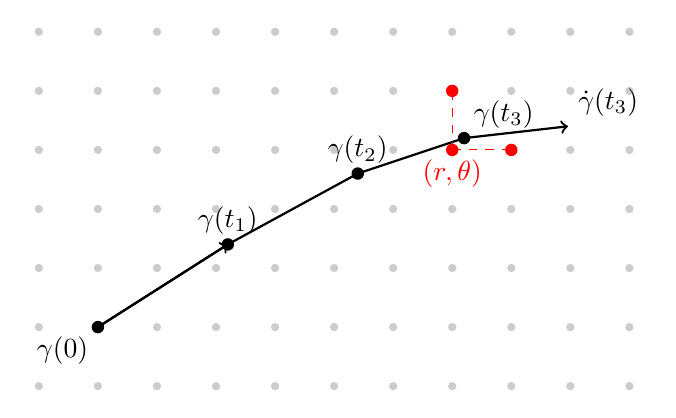
\begin{tikzpicture}[scale=1.5]
    % Grid of dots
    \foreach \x in {0, 0.5, ..., 5} {
        \foreach \y in {0, 0.5, ..., 3} {
            \fill[gray!40] (\x, \y) circle (1pt);
        }
    }
    
    % Path for gamma (smooth curve)
    \draw[thick] plot coordinates {(0.5, 0.5) (1.6, 1.2) (2.7, 1.8) (3.6, 2.1)};
    
    % Gamma points
    \fill (0.5, 0.5) circle (1.5pt) node[below left] {$\gamma(0)$};
    \fill (1.6, 1.2) circle (1.5pt) node[above] {$\gamma(t_1)$};
    \fill (2.7, 1.8) circle (1.5pt) node[above] {$\gamma(t_2)$};
    \fill (3.6, 2.1) circle (1.5pt) node[above right] {$\gamma(t_3)$};
    
    % Initial velocity
    \draw[->, thick] (0.5, 0.5) -- ++(1.1, 0.7);
    
    % Current vector \dot\gamma
    \draw[->, thick] (3.6, 2.1) -- ++(0.88, 0.1) node[above right] {$\dot\gamma(t_3)$};
    
    % Nearest grid point
    \fill[red] (3.5, 2) circle (1.5pt) node[below, text=red] {$(r,\theta)$};
    \fill[red] (4.0, 2) circle (1.5pt);
    \fill[red] (3.5, 2.5) circle (1.5pt);
    
    % Dashed line for first differences
    \draw[dashed, red] (3.5, 2) -- (4, 2);
    \draw[dashed, red] (3.5, 2) -- (3.5, 2.5);
    
\end{tikzpicture}
\end{center}



\end{document}